\normaltrue
\correctionfalse

%\UPSTIidClasse{12} % 11 sup, 12 spé
%\newcommand{\UPSTIidClasse}{12}

\exer{Banc d'essai de Boite de Transfert Principale d'hélicoptère$\star$ \label{C2:10:Coh:530}}
\setcounter{numques}{0}
\UPSTIcompetence[2]{C2-10}
\index{Compétence C2-10}
\index{Torseur de cohésion}
\index{Diagramme des efforts intérieurs}

\ifcorrection
\else
\textbf{Pas de corrigé pour cet exercice.}
\fi

On s'intéresse à la conception d'un banc d'essai de boite de transfert principale d'hélicoptère. 



\begin{obj}
\begin{itemize}
\item Dimensionner l’arbre en sortie de la BTP qui fera la jonction avec le banc d’essai.
\item Déterminer les roulements qui assureront la liaison entre l’arbre 1 et le support S.
\item Concevoir la liaison pivot entre l’arbre de sortie et le bâti.
\end{itemize}
\end{obj}

Dans le cadre d’un essai de la BTP, les pales ne sont pas utilisées. Il est donc nécessaire de concevoir un arbre de sortie qui doit faire office de rotor principal. Cet arbre de sortie devra supporter des efforts équivalents à ceux engendrés par les efforts aérodynamiques. L’accouplement avec le reste du banc d’essai doit permettre de fournir un couple résistant. Par ailleurs, des vérins permettent de générer l’effort de portance. Une modélisation de l’arbre de sortie de la BTP est présentée sur la figure suivante.

 
\begin{center}
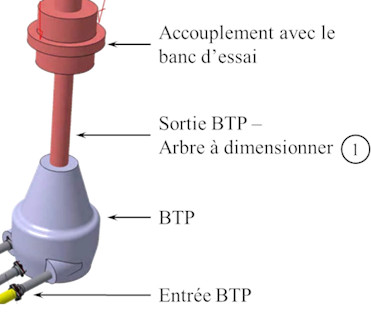
\includegraphics[width=.75\linewidth]{530_01}

\textit{Vue 3D de la BTP et du banc d’essai (système de mise en effort non représenté)}
\end{center}


\begin{center}
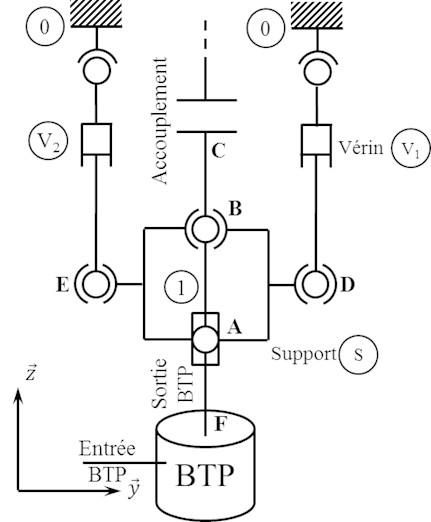
\includegraphics[width=.75\linewidth]{530_02}

\textit{Schéma d’architecture de la sortie de la BTP}
\end{center}



 

On considère un essai dans lequel l’arbre \textbf{1} est sollicité par un effort généré par le vérin V1. On fait les hypothèses suivantes :
\begin{itemize}
\item l’action du vérin $V_1$ sur l’arbre 1 est transmise par l’intermédiaire du support S. L’action du vérin sur le support S est modélisable par un glisseur passant par le point D : $\vect{R}\left( V_1\to S\right)$ avec $F_v=\SI{80 000}{N}$;
\item l’action de la BTP sur l’arbre 1 est un couple $\vect{M}\left(A,\text{BTP}\to 1 \right)=C_1 \vect{z}$ avec $C_1=\SI{4 100}{Nm}$;
\item on considère que les liaisons en $A$ et $B$ sont parfaites, l’accouplement permet donc de transmettre le couple fourni par la BTP ;
\item la pesanteur est négligée.
\end{itemize}
On a :
\begin{itemize}
\item $\vect{AB}=l\vect{z}$ avec $l=\SI{200}{mm}$;
\item $\vect{BD}=L\vect{y}-\dfrac{l}{2}\vect{z}$ avec $L=\SI{300}{mm}$.
\end{itemize}

\subsection*{Dimensionnement de l’arbre}
\begin{obj}	Déterminer le diamètre minimal de l’arbre et son matériau.
\end{obj}

La modélisation retenue pour déterminer le diamètre de l’arbre est la suivante  :
\begin{itemize}
\item l’arbre est modélisé par une poutre cylindrique de révolution de longueur $H$. Une section de la poutre est repérée par l’abscisse $z$ suivant l’axe $(C,\vect{z})$. On note $\vect{CG}=z\vect{z}$;
\item l’action des vérins est modélisée par un seul effort : $F_v \vect{z}$ ;
\item le couple moteur est modélisé par un moment : $C_1\vect{z}$.
\end{itemize} 

\begin{center}
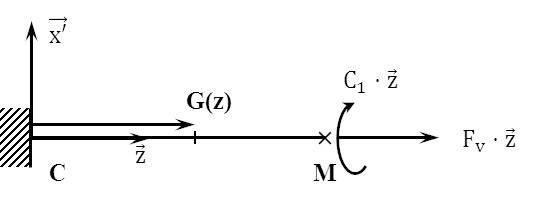
\includegraphics[width=.75\linewidth]{530_03}

\textit{Modélisation des efforts sur l’arbre de sortie de la BTP}
\end{center}

\question{Exprimer le torseur de cohésion en chaque section de la poutre.  À quel(s) type(s) de sollicitation(s) l’arbre est-il soumis ?}
\ifprof
\begin{corrige}~\\
\end{corrige}
\else
\fi

On considère que l’arbre n’est soumis qu’à de la torsion pure.
On note :
\begin{itemize}
\item $\tau_{\text{Max}}$ : la contrainte tangentielle de cisaillement maximale en MPa ;
\item $I_0$ : le moment quadratique polaire en $\text{mm}^4$ ;
\item $d$ : le diamètre de l’arbre en mm.
\end{itemize}
%On a alors τ_Max=C_1/I_0 ⋅d/2 avec I_0=(πd^4)/32.
%La condition de résistance en torsion de l’arbre est donnée par τ_Max<(K⋅R_e)/s avec :
On note :
\begin{itemize}
\item $K$ : coefficient dépendant du type de matériau;
\item $R_e$ : limite élastique à la traction (en MPa);
\item $s$ : coefficient de sécurité.
\end{itemize}

La condition de résistance en torsion peut éventuellement s'écrire $\tau_{\text{max}}< \dfrac{K R_e}{ s}$.

\begin{center}
\begin{tabular}{p{2cm}lp{1.5cm}}
\hline
Famille de matériaux & Pourcentage de carbone & K \\ \hline \hline
Aciers & Inférieur à 0,2 \%	&0,5 \\ \hline
&Entre 0,2 \% et 0,32 \%	&0,6 \\ \hline
&Entre 0,32 \% et 0,45 \%	&0,7 \\ \hline
&Entre 0,45 \% et 1,7 \%	&0,8 \\ \hline
Fonte&Supérieur à 1,7 \%	&Entre 0,77 et 1 \\ \hline
\end{tabular}
\end{center}


\question{On recommande un coefficient de sécurité $s=1,2$. À partir des données précédentes, exprimer de manière littérale quel doit être le diamètre minimum de l’arbre.}
\ifprof
\begin{corrige}~\\
\end{corrige}
\else
\fi

\question{En utilisant l’annexe, donner une liste des matériaux présentant le meilleur compromis prix - résistance élastique.}% Proposer un procédé de mise en forme du brut et un procédé de finition permettant de fabriquer l’arbre de sortie de la BTP.}
\ifprof
\begin{corrige}~\\
\end{corrige}
\else
\fi

\question{On choisit un acier dont la teneur en carbone est comprise entre 0,32\% et 0,45\%. On prendra $R_e=\SI{1 000}{MPa}$ . Déterminer le diamètre de l’arbre.}
\ifprof
\begin{corrige}~\\
\end{corrige}
\else
\fi


\begin{center}
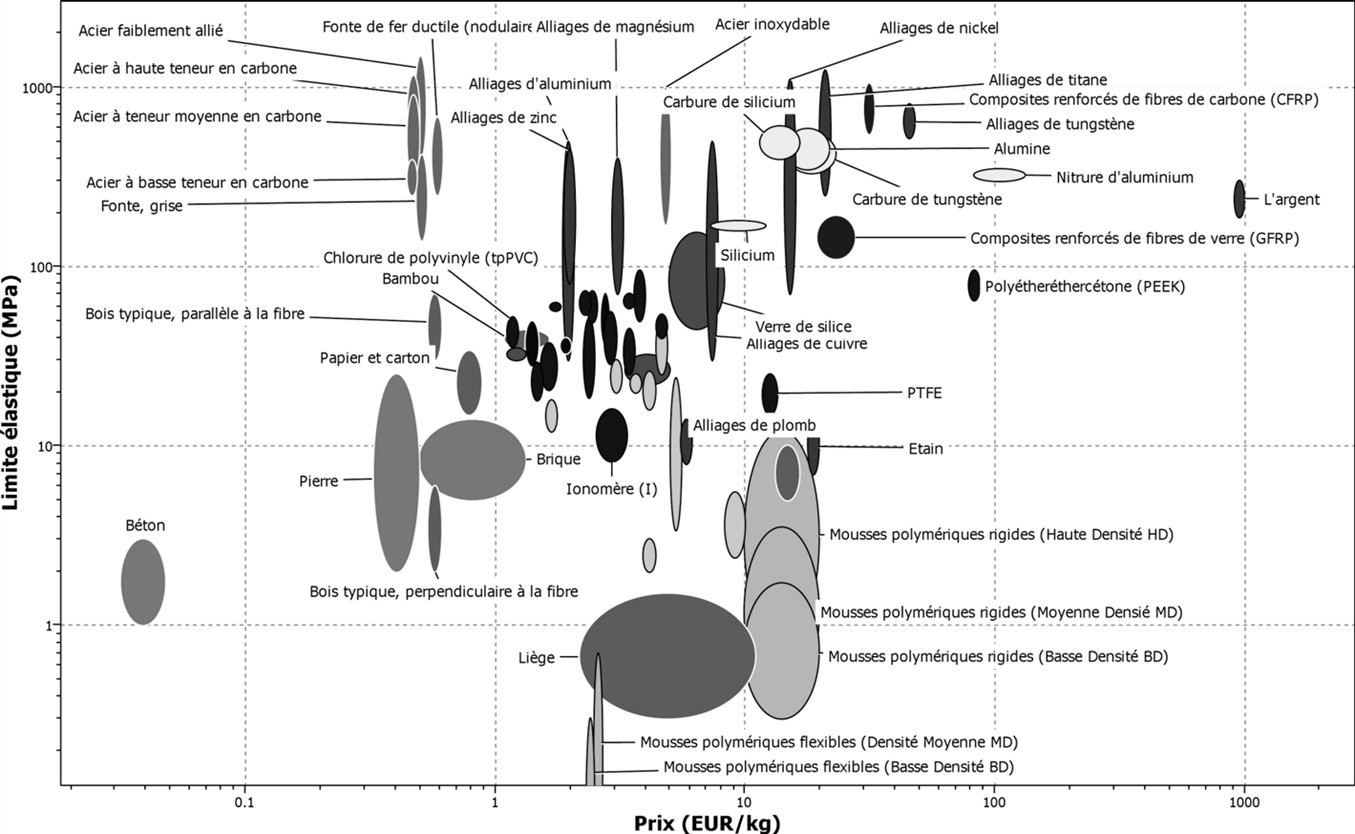
\includegraphics[width=\linewidth]{530_04}
\end{center}


\ifprof
\else
\begin{flushright}
\footnotesize{Corrigé  voir \ref{C2:10:Coh:530}.}
\end{flushright}%
\fi

